%% 
%% Created in 2018 by Martin Slapak
%% last update:		2020-02-09
%%
%% Based on file for NRP report LaTeX class by Vit Zyka (2008)
%% enhanced for MI-MVI (2018) and tuned for BI-PYT (2020)
%%
%% Compilation:
%% >pdflatex report
%% >bibtex report
%% >pdflatex report
%% >pdflatex report

\documentclass[czech]{pyt-report}

\usepackage[utf8]{inputenc}
\usepackage{minted}

\title{Aplikace pro správu dotazníkových šetření}

\author{Lukáš Paukert}
\affiliation{ČVUT -- FIT}
\email{paukeluk@fit.cvut.cz}

\def\file#1{{\tt#1}}

\begin{document}

\maketitle

%%%%%%%%%%%%%%%%%%%%%%%%%%%%%%%%%%%%%%%%%%%%%%%%%%%%%%%%%%%%%%%%%%%%%%%%%%%%%%%%
\section{Úvod}

Tento report vznikl v~rámci semestrální práce v~předmětu BI-PYT.21 v~akademickém roce 2020/2021. Téma semestrální práce je „Webová aplikace pro~dotazníky“.

Cílem práce je vytvořit webovou aplikaci na~správu dotazníkových šetření včetně rozhraní pro~vyplňování respondenty. Důležitou součástí aplikace je také vizualizace nad~výsledky ve~formě grafů. Celé znění zadání je k~dispozici na~stránce předmětu na~Courses.

%%%%%%%%%%%%%%%%%%%%%%%%%%%%%%%%%%%%%%%%%%%%%%%%%%%%%%%%%%%%%%%%%%%%%%%%%%%%%%%%
\section{Využité frameworky a knihovny}

Pro vytvoření aplikace jsem si vybral framework Django, který se řadí mezi~nejpoužívanější webové python frameworky\cite{jetbrains_survey}. Na zobrazování interaktivních grafů využívám knihovnu Plotly a pro generování PDF souborů knihovnu ReportLab.

%%%%%%%%%%%%%%%%%%%%%%%%%%%%%%%%%%%%%%%%%%%%%%%%%%%%%%%%%%%%%%%%%%%%%%%%%%%%%%%%
\section{Struktura databáze}

Jednou z~prvních věcí, kterou si bylo potřeba rozmyslet, je způsob uložení dat. Vzhledem k~potřebě umožnit uživatelům vytvořit dotazník s~libovolným počtem otázek, které mohou obsahovat libovolný počet možností, jsem se rozhodl data ukládat způsobem znázorněným na Obrázku \ref{fig:db-schema}. Můžeme si tedy všimnout 1:N vazby mezi \texttt{poll} a~\texttt{question}, stejně tak mezi \texttt{question} a~\texttt{option}. Odpověď respondenta se ukládá formou jednoho záznamu (\texttt{answer}), který obsahuje cizí klíč na~\texttt{poll}, a~jednotlivých částí odpovědi, které se váží k~daným \texttt{option}. Ty se do~databáze ukládají pouze v~případě, že respondent danou \texttt{option} vybral nebo k~ní napsal textovou odpověď.

\begin{figure}[h]
  \centering\leavevmode
  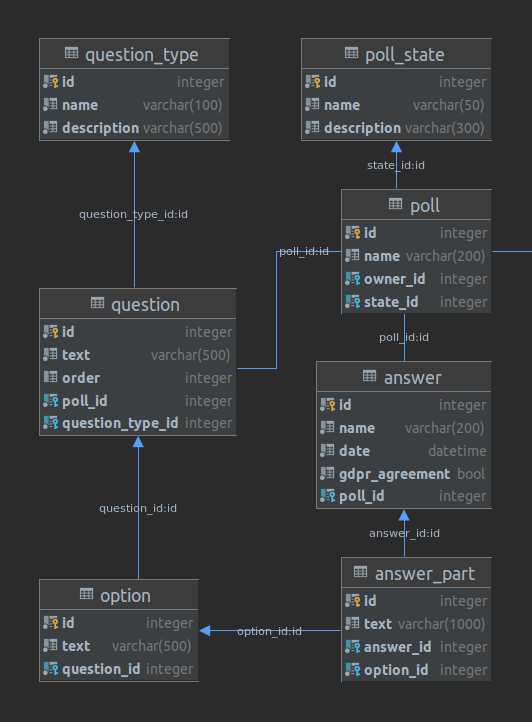
\includegraphics[width=.9\linewidth]{img/db-structure.png}\vskip-0.2cm
  \caption{Schéma databáze}
  \label{fig:db-schema}
\end{figure}

%%%%%%%%%%%%%%%%%%%%%%%%%%%%%%%%%%%%%%%%%%%%%%%%%%%%%%%%%%%%%%%%%%%%%%%%%%%%%%%%
\section{Popis aplikace}

Pro~správné fungování aplikace je před~prvním spuštěním potřeba inicializovat databázi pomocí příkazu \texttt{python manage.py migrate}. Pro~jednoduché vyzkoušení aplikace jsou v~souboru \texttt{dml.sql} připraveny dvě testovací ankety, které je možné do~databáze také vložit.

\subsection{Autentizace}
Před~vytvořením první ankety je potřeba si vytvořit uživatelský účet. Pro~jednoduchost nejsou vyžadovány žádné osobní údaje kromě uživatelského jména a hesla, pomocí nichž bude uživatel přistupovat do~administrátorského rozhraní.\footnote{Toto zjednodušení má samozřejmě za~následek to, že například není možné heslo obnovit, což by v~reálné aplikaci byla jistě žádaná funkčnost.}

\subsection{Vytvoření a správa ankety}
Po~přihlášení může uživatel v administrátorském rozhraní vytvořit anketu a~následně z~rozhraní pro~úpravu anket je možné přidávat otázky a~k~nim jednotlivé možnosti. Pro~všechny typy otázek (\texttt{Single choice}, \texttt{Multi choice} i~\texttt{Text answer)} jsem se rozhodl umožnit vkládat libovolný počet možností. To u~otázek s~textovou odpovědí znamená více políček pro~textovou odpověď viz připravené ankety v~\texttt{dml.sql}. Po~výše zmíněných krocích je anketa ve~stavu \texttt{Draft} a není přístupná respondentům. Pro~zpřístupnění je třeba na~stránce pro~úpravu ankety stisknout tlačítko \texttt{Start poll}, které ji přepne do~stavu \texttt{Active}. V~tomto stavu je možné anketu vyplňovat, avšak již není umožněno její obsah jakkoliv upravovat. Oproti zadání jsem se rozhodl i~v~tomto stavu ankety umožnit zobrazení výsledků a~i~jejich případný export. Pro~uzavření průzkumu je potřeba opět na~stejné stránce kliknout na tlačítko \texttt{Close poll}.

\subsection{Vyplňování ankety respondenty}
Samotné vyplnění ankety je možné po~zadání jejího kódu na~hlavní stránce aplikace nebo~přes~obdržený odkaz.\footnote{V~současné verzi aplikace se kód ankety rovná jejímu ID. Toto by bylo dobré určitě upravit, aby případné \emph{soukromé} ankety nemohl vyplňovat kdokoliv.} Každá anketa obsahuje políčko pro~jméno respondenta, které je jistě osobním údajem. Proto tento údaj bude uložen do databáze pouze v~případě, že respondent dá souhlas se zpracováním osobních údajů. Po~domluvě se cvičícím ve~své práci neřeším zpracování případně dalších osobních údajů, které by mohly být součástí jakékoliv otázky.

\subsection{Výsledky}
Jak už jsem zmínil dříve, výsledky ankety je možno zobrazit v~jakémkoliv jejím stavu. Pokud zatím žádný respondent anketu nevyplnil, je administrátorovi zobrazena příslušná informace. Je umožněno zobrazit odpovědi jednotlivých respondentů i~celkový přehled odpovědí. V~něm jsou pro přehlednost výsledky ankety znázorněny pomocí grafů. Odpovědi na~\texttt{Single choice} otázky jsou reprezentovány pomocí kruhového (koláčového) grafu, na~\texttt{Multi choice} otázky pomocí sloupcovitého grafu. Odpovědi na~textové otázky jsou zobrazeny bez~dalšího znázornění. Všechny grafy jsou díky využité knihovně Plotly interaktivní. Pro~další zpracování výsledků je možné také využít připravený export do~CSV formátu.

\subsection{Ostatní funkcionality}
\begin{itemize}
\item pro~případ, že by anketu nebylo možné vyplňovat na~počítači, je připraven export ankety do~PDF souboru
\item anketu (její název, otázky a~jednotlivé možnosti) je možné z~aplikace exportovat a do~aplikace importovat jako CSV soubor. Po importu bude daná anketa nastavena do~stavu \texttt{Draft} a~je ji tedy možné ještě doupravit přímo v~aplikaci.
\end{itemize}

%%%%%%%%%%%%%%%%%%%%%%%%%%%%%%%%%%%%%%%%%%%%%%%%%%%%%%%%%%%%%%%%%%%%%%%%%%%%%%%%
\section{Závěr}

Při~práci na~tomto projektu jsem asi poprvé pracoval s~nějakým frameworkem a za~tuto zkušenost jsem velice rád. S~výslednou aplikací jsem spokojený, ale určité věci by samozřejmě šly ještě vylepšit.

Některá možná vylepšení jsem již zmínil dříve, jako další bych například uvedl vylepšení logiky pro~úpravu anket. V~současné verzi dojde při~stisknutí jakéhokoliv tlačítka (např.~pro~přidání/odebrání otázky) k~uložení celého dotazníku, ale toto chování nemusí být vždy žádoucí. S tím souvisí nevyužití \texttt{Django formulářů}, o~kterých jsem se dozvěděl bohužel pozdě. Dále by šlo jistě vylepšit celkový vzhled aplikace, například s~využitím nějakého frameworku jako je Bootstrap.

%%%%%%%%%%%%%%%%%%%%%%%%%%%%%%%%%%%%%%%%%%%%%%%%%%%%%%%%%%%%%%%%%%%%%%%%%%%%%%%%

%\bibliographystyle{plain-cz-online}
\bibliography{reference}

\end{document}
